% 矢量叉乘分配律的几何证明
% 线性代数|矢量|叉乘|cross product|叉积|cross product|向量积|vector product|矢量积|分配率|投影

\pentry{矢量的叉乘\upref{Cross}}
证明 $\bvec A \cross (\bvec B + \bvec C) = \bvec A \cross \bvec B + \bvec A \cross \bvec C$ 

\begin{figure}[ht]
\vskip-10pt
\centering
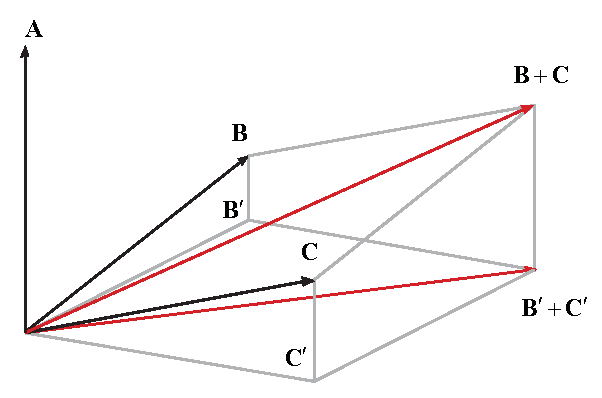
\includegraphics[width=8.5cm]{./figures/CrossP1.pdf}
\caption{把 $\bvec B,\bvec C,\bvec D$ 投影到与 $\bvec A$ 垂直的平面上}
\end{figure}

首先令
\begin{equation}
\bvec D = \bvec B + \bvec C
\end{equation}
把矢量 $\bvec B,\bvec C,\bvec D$ 在与矢量 $\bvec A$ 垂直的平面上投影,分别得到 $\bvec B',\bvec C',\bvec D'$. 显然,$\bvec D'=\bvec B'+\bvec C'$. 

现在先证明
\begin{equation}
\bvec A \cross \bvec B = \bvec A \cross \bvec B'
\end{equation} 
这是叉乘的一个基本的性质.首先,
根据叉乘的几何定义\upref{Cross}, $\bvec A \cross \bvec B$ 与
 $\bvec A \cross \bvec B'$ 的方向相同.另外
\begin{equation}
\abs{\bvec A \cross \bvec B}  = \abs{\bvec A} \abs{\bvec B} \sin{\theta_{AB}} = \abs{\bvec A} \abs{\bvec B'}=\abs{\bvec A \cross \bvec B'}
\end{equation}
所以二者模长也相等,证毕.

同理有 
\begin{equation}
\bvec A \cross \bvec C = \bvec A \cross \bvec C'
\end{equation}
\begin{equation}
\bvec A \cross \bvec D = \bvec A \cross \bvec D'
\end{equation}
所以,要证明
\begin{equation}
\bvec A \cross \bvec D = \bvec A \cross \bvec B + \bvec A \cross \bvec C
\end{equation}
只需要证明
\begin{equation}
\bvec A \cross \bvec D' = \bvec A \cross \bvec B' + \bvec A \cross \bvec C'
\end{equation}
即可.

由于 $\bvec B', \bvec C', \bvec D'$ 都与 $\bvec A$ 垂直,所以 $\bvec A$ 与之叉乘的效果相当于 $\bvec B', \bvec C', \bvec D'$ 的模长分别乘以 $\abs {\bvec A}$, 且绕 $\bvec A$ 逆时针分别旋转 $90°$. 所以上式就是在说, 若已知 $\bvec B' + \bvec C' = \bvec D'$, 那么把它们分别乘以常数并旋转 $90°$ 后这个加法仍然成立. 这是显然的. 证毕.
